\chapter{Konzept}
In diesem Kapitel wird zunächst erläutert, wie die Steuerung der Getränkemischmaschine durch Sprachbefehle im Allgemeinen ablaufen wird.
Anschließend werden mehrere Konzepte vorgestellt, die das allgemeine Konzept konkretisieren.
Diese werden anhand der, in Kapitel \ref{section:Bewertungskriterien} erläuterten Kriterien, bewertet.
Zuletzt wird die Wahl des finalen Konzepts begründet.
\section{Allgemein}
Der Benutzer soll über Spracheingaben mit der Mischmaschine interagieren können.
Dafür muss das Gesprochene zunächst durch ein Mikrofon aufgenommen werden.
Anschließend können die Audiosignale weiterverarbeitet werden.
Der Benutzer soll hierbei nicht auf fest vorgegebene Sprachbefehle beschränkt sein, sondern für nahezu jede Eingabe eine sinnvolle Antwort zurückerhalten.
Um dies zu gewährleisten wird die Spracheingabe durch ein Sprachmodell, welches mittels maschinellen Lernverfahren trainiert wurde, verarbeitet. 
Ergebnisse dieser Verarbeitung sind die Antwort, die an den Benutzer zurückgegeben wird, und ein konkreter Befehl für die Mischmaschine.
Ein Beispiel für einen solchen Befehl könnte etwa die Zubereitung eines bestimmten Getränks sein.
Für die Ausgabe einer Antwort ist ein Lautsprecher notwendig.
Denkbar wäre auch eine textbasierte Ausgabe, allerdings ginge damit der Eindruck des Benutzers verloren eine echte Konversation mit der Mischmaschine zu führen.
Das Sprachmodell mit der Getränkemischmaschine zu verknüpfen stellt eine Herausforderung dieser Arbeit dar.
\section{Bewertungskriterien} \label{section:Bewertungskriterien}
Im Folgenden sind die Bewertungskriterien für die einzelnen Konzepte aufgelistet:
\begin{itemize}
    \item Freiheitsgrade in der Spracheingabe des Benutzers
    \item Hardwarekosten
    \item Verfügbare Rechenleistung
\end{itemize}
\section{Konzept A: Spracherkennung und -verarbeitung mittels Arduino}
Ein erstes Konzept sieht vor, dass das Audiosignal direkt von einem der Arduinos in der Getränkemischmaschine aufgenommen wird.
\begin{figure}[H]
    \centering
    % \includegraphics does not allow jpg images apparently!
    \fbox{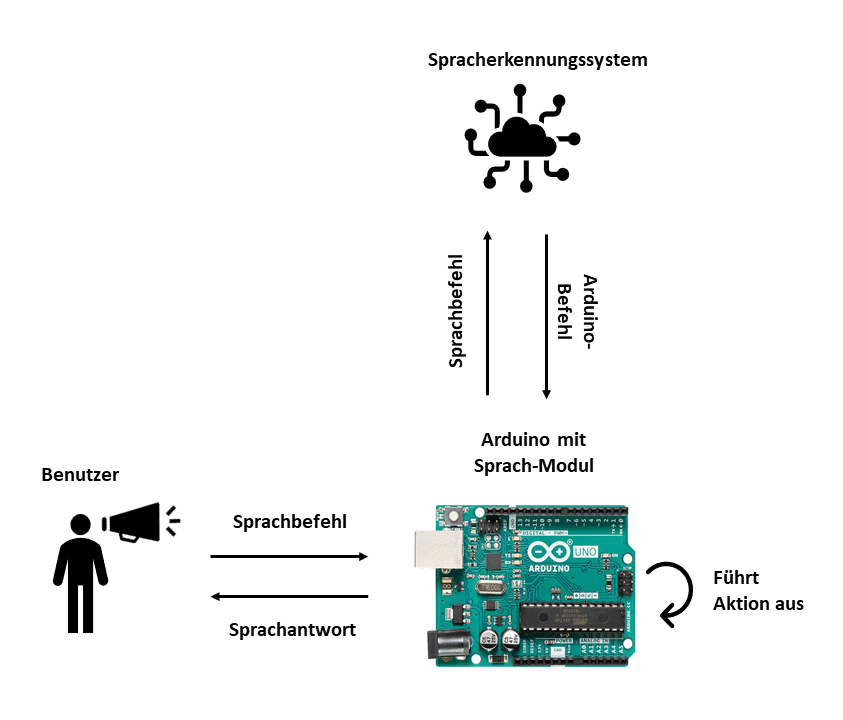
\includegraphics[width=0.8\textwidth]{Bilder_Kapitel_3/Konzept_A.png}}
    \caption{\label{figure:Spracherkennung_mittels_Arduino}Spracherkennung und -verarbeitung mittels Arduino}
\end{figure}
\section{Konzept B: Spracherkennung und -verarbeitung mittels mobiler Anwendung}
\section{Konzept C: Spracherkennung und -verarbeitung auf Computer-Hardware}
\section{Konzept D:}
\section{Finales Konzept}
\endinput



